\chapter{Results}

\section{ML models results}
In section \ref{section:ML_models} was described the construction of several ML models aimed at predicting ferromagnetic materials critical temperature based exclusively on their chemical composition. The final summary of the best models’ performance in comparison with reference work is presented in table~\ref{tab:best_models_summary}. 

\begin{table}[H]
\centering
\caption{Summary of the best ML models performance}
\begin{tabular}{|p{2.5cm}|p{1.6cm}|p{1.6cm}|p{1.6cm}|p{1.6cm}|p{1.6cm}|p{1.8cm}|}
\hline 
Metrics & SISSO & KRR & RF & XGB & RF (ref.) & KRR (ref.) \\ 
\hline 
$R^2 (test)$ & 0.618 & 0.793 & 0.833 & 0.845 & 0.87 & 0.72 \\ 
$R^2 (cross.val)$ & - & 0.787 & 0.828 & 0.837 & 0.81 & - \\ 
MAE (K) & 138 & 84 & 71 & 69 & 57 & - \\ 
RMSE (K) & 171 & 121 & 109 & 105 & - & - \\ 
Max Error (K) & 761 & 642 & 516 & 595 & - & - \\ 
\hline 
\end{tabular} 
\label{tab:best_models_summary}
\end{table}

The highest accuracy demonstrated by the XGBoost model with $R^2$ and mean absolute error of 0.845 and 69 K respectively on the test set. But the lowest maximum error is shown by the RF.
It is worth to mention that descriptors used in this work are different from the one used in the reference. 
A serious drawback of considered features is the absence of any structural information which makes it impossible to distinguish between two compositions with similar stoichiometry. But after all this work might be considered as a second small step (after ref.  \cite{Nelson:2019ui} toward the ML-driven computational search for novel magnetic materials.

All the generic python code produced in this part of the work stored at GitHub repository (\url{https://github.com/Volkov-da/curie_calculator/tree/master/ML_model}).
The whole process of data cleaning, preprocessing as well as model training and validation stored in a form of briefly commented jupyter-notebook (file \textit{ML\_training.ipynb}).

The pipline showed the best performance (MinMaxScaler + XGBoost) was additionaly retrained over the entire dataset and stored in easy reproducible JSON format.



\section{DFT calculations results}
Using the framework described in section \ref{section: DFT_MC} were calculated values of critical temperature for 20 binary structures containing pure metals, oxides, borides, etc., and 2 gadolinium containing ternary structures.  Obtained values were compared with experimental ones as well as with the results from the theoretical calculations of other groups. Relative error was calculated as follows:

\begin{equation}
\Delta = \frac{\left| T_{exp} - T_{DFT} \right|}{T_{exp}}
\end{equation}

As it might be seen from the table \ref{tab:gga_summary} in general GGA + U approach outperforms GGA.  Mean relative error for the unary structures in the case of GGA is 39.5\% for GGA + U is 30.9\%, for oxides 40.4\% and 33.5\%,  for other binary structures (borides, etc.) it is 42.4\% and 25.1\% respectively. 

From the plot \ref{fig:gga} we may conclude that in general GGA tends to underestimate critical temperature with the exclusions of 4 structures, namely: \textit{MnO}, \textit{NiO}, \textit{MnAs}, \textit{EuS}. 

\begin{figure}[H]
\centering
\captionsetup{justification=centering,margin=2cm}
	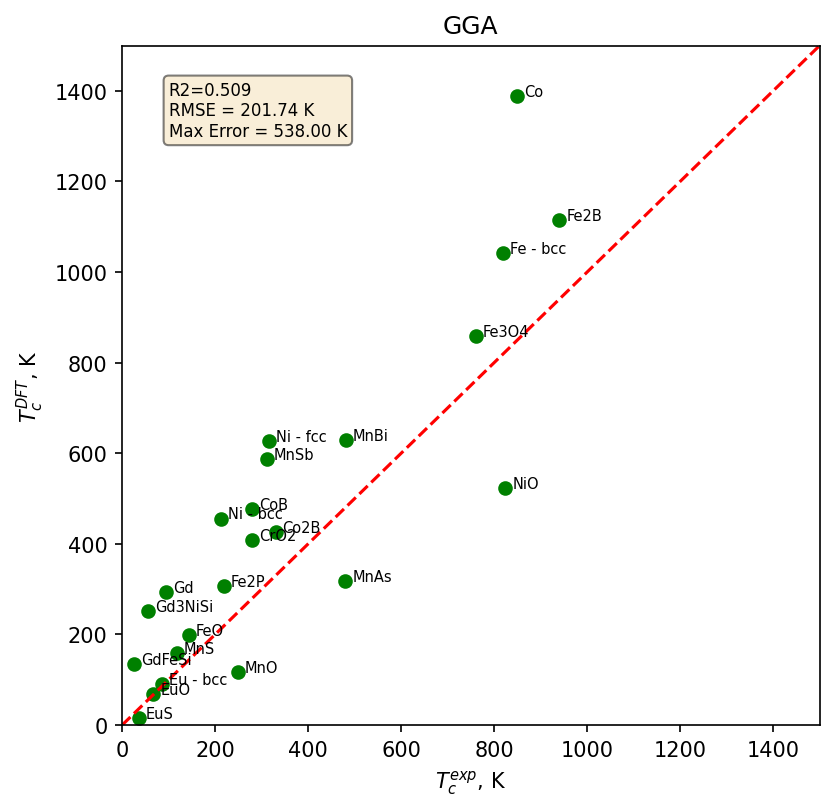
\includegraphics[width=80mm]{fig/dft_fig/gga_results.png}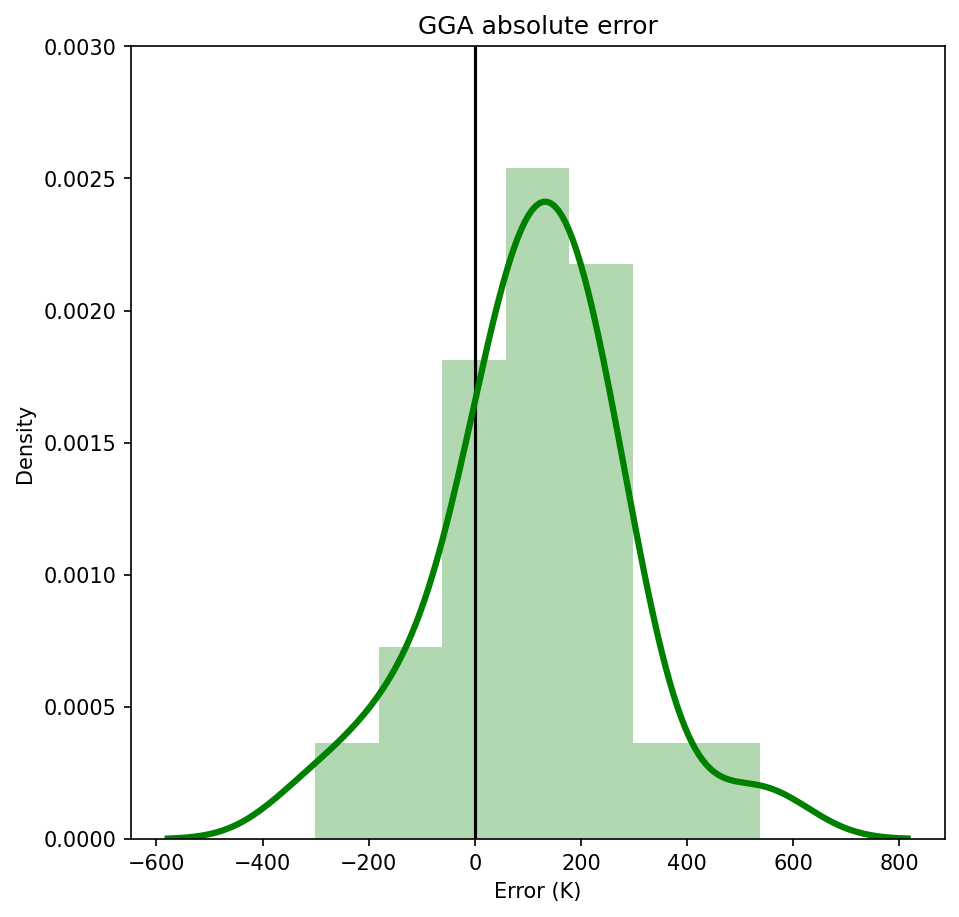
\includegraphics[width=80mm]{fig/dft_fig/gga_err.png}
	\caption[Comparison of calculated by GGA results with experimental.]{Left: Comparison of calculated by GGA results with experimental. Right: Absolute errors distribution.}
\label{fig:gga}
\end{figure}

 Maximum relative errors of  125 \% are shown in the case of \textit{EuS}, but anyway, the resulting value we may consider pretty reasonable due to the small absolute difference ($16\ K$ and $36\ K$ respectively).  A maximum absolute error of $538\ K$ appears in the case of cobalt, the FM material with the highest known critical temperature.  The lowest absolute difference in calculated and experimental values was shown by three Eu containing structures its $5\ K$ for \textit{Eu-bcc}, $20\ K$ for \textit{EuS} and $2\ K$ for \textit{EuO} which is so far also the material with the lowest relative error of only 5.5\%.



Results obtained during the GGA+U calculations presented in figure \ref{fig:gga_u}.  The distribution of errors is closer to zero compared to GGA results, and there is no clear tendency towards over/under- estimation of Curie point.  Maximum relative error of 53.4\% in this case shown by \textit{MnO}, while a bit bigger maximum absolute error of $608\ K$ once again by cobalt.  Lowest absolute difference of $15K$ and $23K$ as well as the lowest relative error of 9.4\% and 11.6\% were shown by \textit{MnS} and \textit{FeO} respectively.  Eu-containing structures were not considered in GGA+U calculations due to the absence of a predefined U value. Once again worth mentioning that due to the automated way of calculating, none of Hubbard correction values was calibrated explicitly. Hence we may expect even better results in the case of proper calibration with a linear response method for each particular structure.

\begin{figure}[H]
\centering
\captionsetup{justification=centering,margin=2cm}
	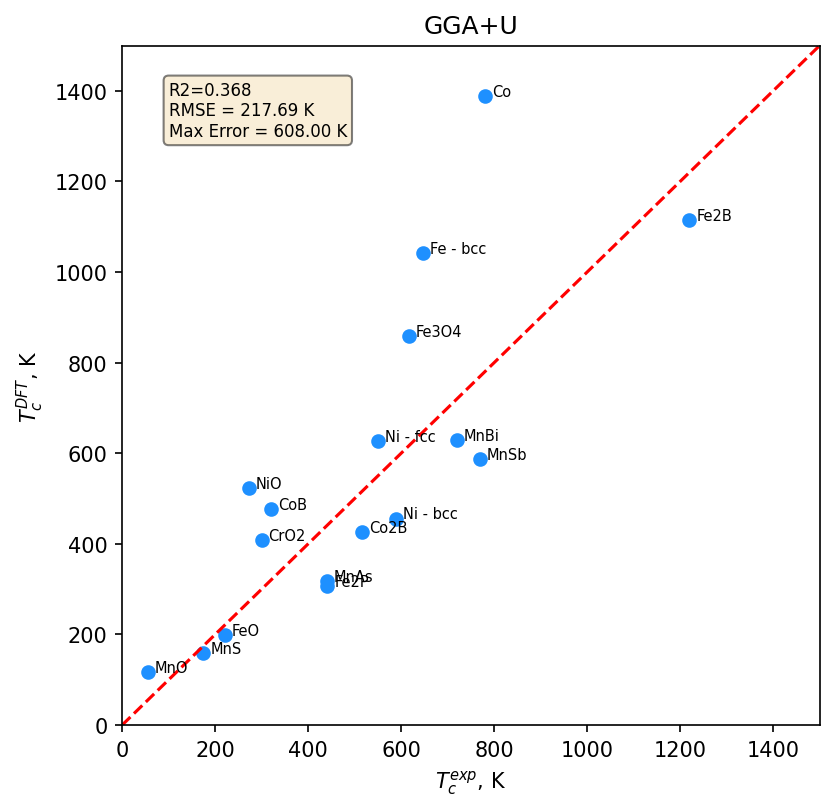
\includegraphics[width=80mm]{fig/dft_fig/gga_u_results.png}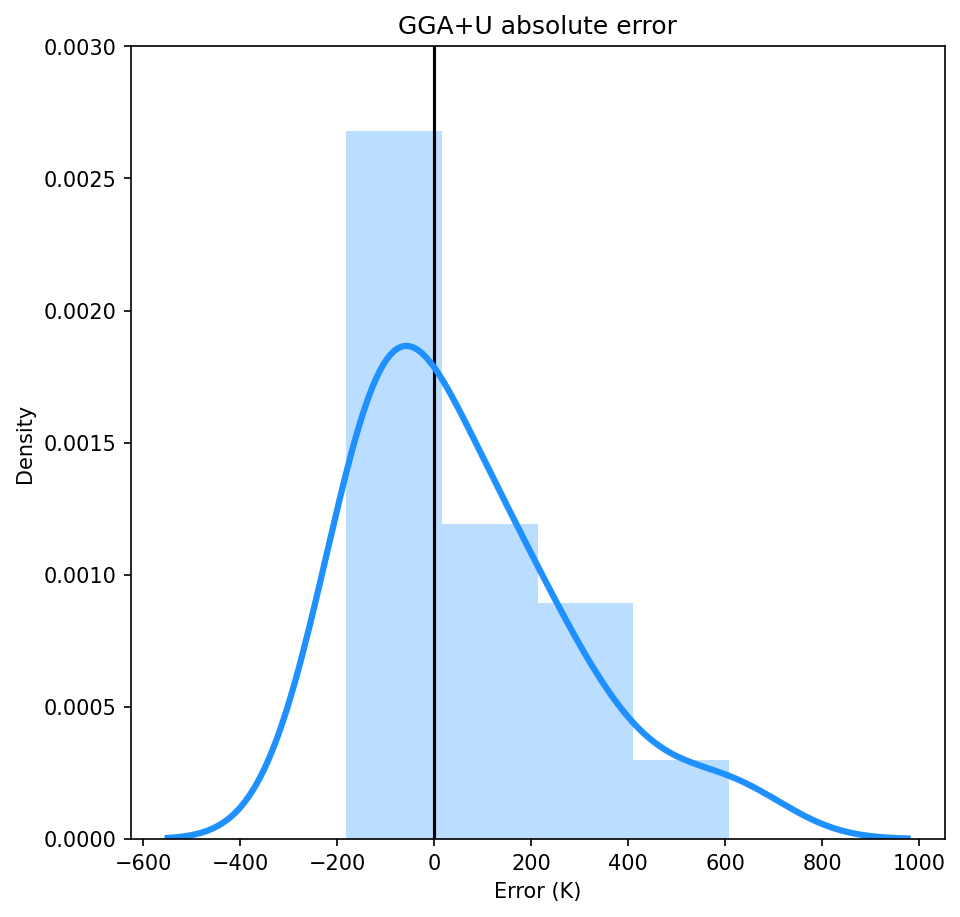
\includegraphics[width=80mm]{fig/dft_fig/gga_u_err.png}
	\caption[Comparison of calculated by GGA+U results with experimental.]{Left: Comparison of calculated by GGA+U results with experimental. Right: Absolute errors distribution.}
\label{fig:gga_u}
\end{figure}


Results obtained during GGA and GGA + U calculations with relative errors compared to the experimental data presented in the table \ref{tab:gga_summary}.  


\begin{table}[H]
\centering
\caption{Comparison of calculated by GGA and GGA+U results with experimental.}
\begin{tabular}{|p{2.6cm}|p{1.6cm}|p{1.6cm}|p{1.6cm}|p{1.6cm}|p{1.6cm}|p{1.6cm}|}
\hline 
\multirow{2}{*}{Material} & \multicolumn{4}{|c|}{$T_C, K$} &\multicolumn{2}{|c|}{$\Delta, \%$}\\\cline{2-7}
 & ref. & exp. & GGA & GGA+U & GGA & GGA+U\\ 
\hline 
Fe-bcc \cite{Pajda_2001} & 950 & 1043 & 820 & 648 & 21.4  & 37.9 \\ 
Co-fcc \cite {Pajda_2001} & 1311 & 1388 & 850 & 780 &  38.8 & 43.8 \\ 
Ni-fcc \cite{Pajda_2001} & 300 & 627 & 315 & 550 & 49.8 & 12.3 \\ 
Ni-bcc \cite{Tian_2005} & 250 & 456 & 212 & 590 & 53.5  & 29.4 \\ 
Gd \cite{Tereshina_2016} & 293 & 294 & 94 &- & 68.0 & - \\ 
Eu-bcc & 111 & 91 & 86 & - & 5.5 & - \\ 
\hline
\ce{EuO} \cite{Jutong_2015} & 35 & 69 & 67 & - & 2.9 & - \\ 
\ce{Fe_3O_4} & - & 858 & 760 & 616 & 11.4  & 28.2 \\ 
\ce{CrO_2} \cite{Huang_2018} & 305 & 408 & 280 & 300 & 31.4  & 26.5 \\ 
MnO \cite{Archer_2011, Roth_1958} & 240  & 118 & 249 & 55 & 111.0 & 53.4 \\ 
NiO \cite{Archer_2011, Roth_1958} & 393 & 523  & 824 & 272 &  57.6 & 48.0 \\ 
\hline 
\ce{Fe2B} \cite{Markus_2015} & 1000 & 1115 & 940 & 1220 & 15.7 & 9.4 \\ 
\ce{Co_2B} \cite{Markus_2015} & 450 & 426 & 330 & 516 &  22.5 & 21.1 \\ 
CoB & 411 & 477 & 280 & 320 &41.3  & 32.9 \\
\ce{Fe_2P} & - & 306 & 219 & 441 & 28.4  & 44.1 \\ 
MnBi & - & 630 & 481 & 720 &  23.7 & 14.3 \\ 
MnSb & - & 587 & 311 & 769 & 47.0 & 31 \\ 
MnAs & - & 318 & 480 & 440 & 50.9 & 38.4 \\ 
EuS \cite{Houten_1962} & - & 16 & 36 & - & 125.0 & - \\ 
\hline 
\ce{Gd_3NiSi2} \cite{Liu_2009} & 215 & 251 & 56 & - & 77.7 & - \\ 
\ce{GdFeSi} & 145 & 135 & 25 & - & 81.5 & - \\ 
\hline 
\end{tabular}
\label{tab:gga_summary}
\end{table}


\section{Novel structures study}

At a final stage of all the performed work develop methods for critical temperature calculations we applied in a direct exploration of newly predicted magnetic structures. As mentioned before, nowadays, it's already possible to perform a computational search of such structures but optimizing them only concerning stability and magnetic moment. So as a final step of this work, a developed in section \ref{section: DFT_MC} algorithm based on DFT + MC calculations and the best-trained ML model from section \ref{section: XGBoost} was applied to benchmark new structures with respect to their Curie temperature.  Namely were tested 55 promising magnetic compositions obtained during coevolutionary (Mendelevian) search as implemented in MendS alghoritm \cite{Allahyari_2020}.


Distribution of estimated critical temperatures presented in the figure \ref{fig:dft_hist}. As it is shown, the correlation between the results produced by the two described methodology is quite weak. Generally, it might be explained due to the nature of the descriptors used in ML model training. Since prepared features were exclusively based on chemical information without considering structural data, the whole predictive model tends to predict high values of critical temperature for the compositions with the close to known in model stoichiometry. Thus even for previously unknown Fe and Co-containing structures ML model always expect values of critical temperature higher than 400~K in the same fashion as for the known from training data compositions containing these elements.


\begin{figure}[H]
	\centering
	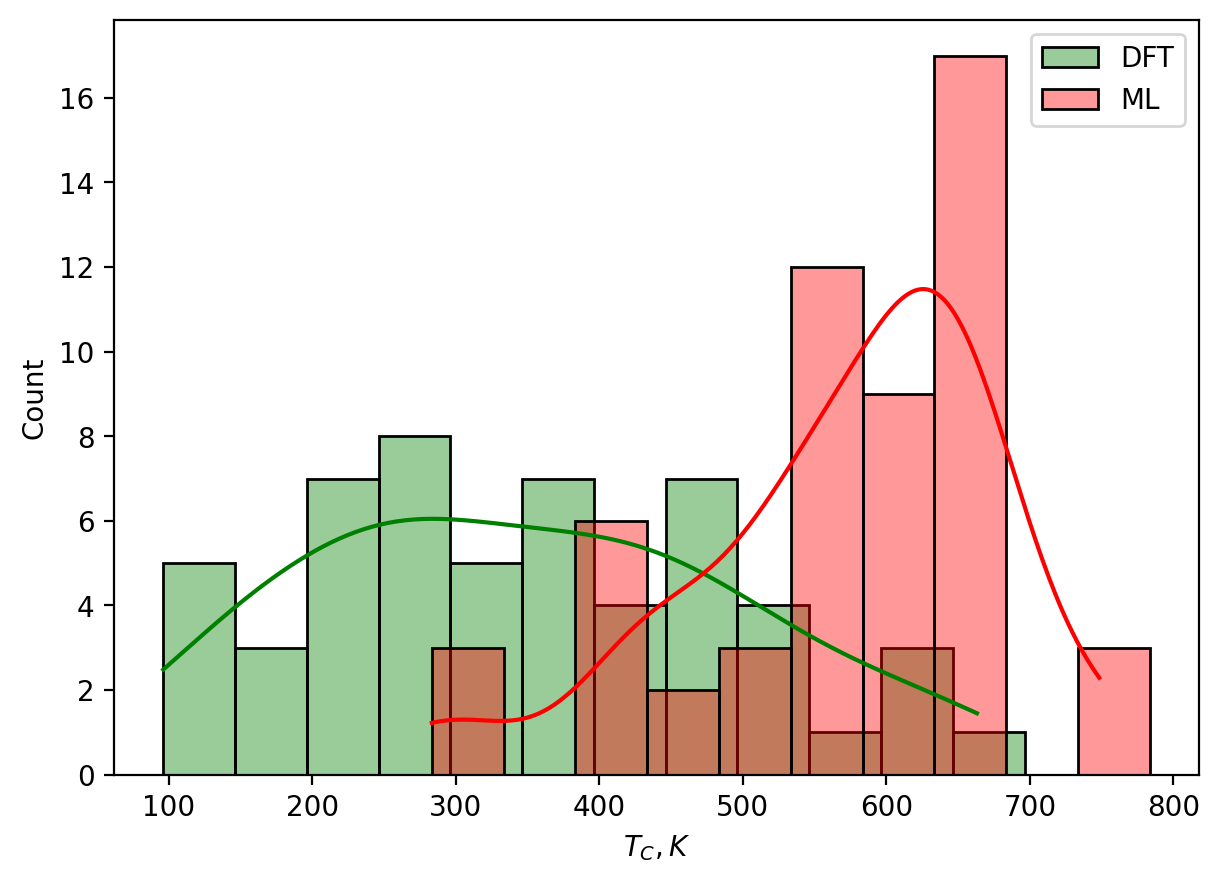
\includegraphics[width=120mm]{fig/dft_fig/ml_dft_hist.png}
	\caption[Histogram of estimated critical temperature using ML and DFT.]{Histogram of estimated critical temperature using ML and DFT.}
\label{fig:dft_hist}
\end{figure}


Estimation given for the new structures by DFT + MC approach (green histogram) has a more uniform distribution and closer in shape to the experimental critical temperature distribution obtained for known FM materials from figure \ref{fig:tc_distrib}. Of course, such a comparison might seem incorrect but intuitively its looks like the more new structures will be tested the more these distributions should have in common.

According to the produced results tree newly predicted structures were classified as a materials with high critical temperature namely $C2/m - Fe_6Mo$   with $T_C^{DFT} = 630 K$ and $T_C^{ML} = 479 K$,  stable $Cmmm - HfCo_5$ with $T_C^{DFT} = 633 K$ and $T_C^{ML} = 425 K$ and metastable $F\bar{4}3m - HfCo_5$ with $T_C^{DFT} = 663 K$ and $T_C^{ML} = 425 K$.


